
El Laboratorio de Mecánica de Fluidos, antes de comenzar con este proyecto utilizaba un archivo Excel para hacer la corrección de la velocidad del aire. En este se calcula matemáticamente la densidad del aire en función de la presión, temperatura y humedad atmosférica.
%	densidad_funcion_P_T_H.pdf  dentro del drive
\begin{align}
	\rho&=\frac{3,48353\;10^{-3}\;kg\;K\;J^{-1}\;\cdot p\cdot\;(1-0,378\;\cdot\;x_v)}{Z\;\cdot\;T} \label{ec_den}\\
	x_v&=\frac{(\alpha+\beta\cdot p+\gamma\cdot t^2)\cdot(1Pa\cdot\;e^{AT^2+BT+C+D/T)})\cdot h/100}p\\
	Z&=\;1-\frac pT\cdot\lbrack a_0+a_1t+a_0t^2+(b_0+b_1t)x_v+(c_0+c_1t)x_v^2\rbrack+(d+x_v^2)\frac{p^2}{T^2}
\end{align}

dónde:\\
- \textbf{p } [Pa] presión atmosférica medida,\\
- \textbf{t } [$^{\circ}$C] temperatura medida,\\
- \textbf{T } [K] temperatura absoluta (\textbf{T}=\textbf{t} + 273,15 \textbf{K})\\
- \textbf{h } [\%] humedad relativa medida,\\
- y constantes \textbf{A,B,C,D,} $\boldsymbol{\alpha , \beta  , \gamma , a_0, a_1 ,a_2 ,b_0  ,b_1 , c_0 , c_1, D. }$


Finalmente, la ecuación anteriormente nombrada es utilizada para el cálculo final de la velocidad del aire.
\begin{equation}
	\triangle P=\frac{v^2\rho}2\rightarrow\;\;v=\sqrt{\frac{2\;.\;\triangle P\;}\rho}
	\label{ec_aire}
\end{equation}

\begin{comment}
Tanto las ecuaciones de densidad ec.(\ref{ec_den})
y la ecuación del cálculo de velocidad  ec.(\ref{ec_aire})
se desarrolló dentro del programa de \textbf{Arduino} para observar como dato final la velocidad del aire.
\end{comment}

En vista al objetivo y a las ecuaciones \ref{ec_den} y \ref{ec_aire} se estableció necesario la obtención de las variables temperatura, presión atmosférica, humedad relativa y diferencia de presión del fluido. 

\subsection{Características del flujo}
La inspección cuidadosa en una tubería revela una corriente de fluidos currentilínea a bajas velocidades y caótica mientras la velocidad aumenta por arriba de un valor crítico. Se dice que el régimen de flujo en el primer caso es laminar, y se caracteriza por líneas de corriente suaves y movimiento sumamente
ordenado; mientras que en el segundo caso es turbulento, y se caracteriza por
fluctuaciones de velocidad y movimiento  desordenado. La mayoría de los flujos que se encuentran en la
práctica son turbulentos. 

\subsubsection{Estimación del número de Reynolds}
\begin{tcolorbox}[colback=blue!5!white,colframe=blue!75!black,title=Número de Reynolds]
	El número de Reynolds (Re) es un número adimensional utilizado en mecánica de fluidos para caracterizar el movimiento de un fluido. Su valor indica si el flujo sigue un modelo laminar o turbulento.
\end{tcolorbox}
El número de Reynolds fue calculado a partir de la ecuación \ref{reyn}, que relaciona las fuerzas inerciales y las fuerzas viscosas. 
\begin{equation}	
	R_e=\frac{\rho\;D_h\;v}\mu
	\label{reyn}
\end{equation}	
dónde:\\
- \textbf{$\rho$ } [$kg/m^{3}$] densidad del fluido \\
- \textbf{$v$ } [$m/s$] velocidad del fluido\\
- \textbf{$D_h$ } [$m$] diametro hidráulico\\
- \textbf{$\mu$ } [$kg/m.s$] viscosidad dinámica del fluido\\

La \textit{densidad del fluido} se calculó con la ecuación \ref{ec_den} vista en la sección \ref{sec:ecvel} con mediciones de temperatura, humedad y presión atmosférica obtenidas con el instrumento \textit{Testo 435}.

La \textit{viscosidad dinámica} del fluido se obtuvo de la tabla "Propiedades del aire a 1 atm de presión" { }del libro \textit{Mécanica de Fluidos} \cite{yunus2006mecanica}.

El \textit{díametro hidráuliaco} de una tubería de sección rectangular es dependiente del valor de sus lados (Figura \ref{fig:rey2} y \ref{fig:camens}) \cite{licci2020estudio}.

Para la \textit{velocidad del fluido} se utilizó un valor de 4,7$m/s$, siendo la velocidad mínima generada por el túnel. Ya que al ser proporcional al número de Reynolds, este será el mínimo valor estimado.

\begin{figure}[htb]
	\centering
	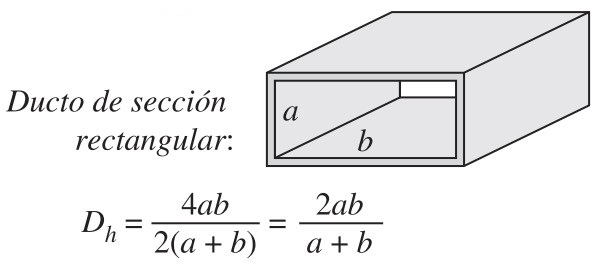
\includegraphics[scale=0.45]{rey2.jpg}
	\captionof{figure}{Diámetro hidráulico}
	\label{fig:rey2}
\end{figure}


\begin{figure}[htb]
	\centering
	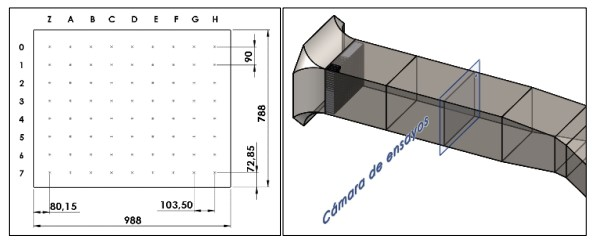
\includegraphics[scale=0.9]{camaraensayos.jpg}
	\captionof{figure}{Dimensiones de la cámara de ensayos en mm}
	\label{fig:camens}
\end{figure}

Si se reemplaza los valores se obtiene:
\begin{equation} 
	R_e\approx \frac{1,193\;kg/m^{3}\;0,86\;m\;4,7\;m/s}{0,000018\;kg/m.s}\approx 270658
	\label{reyn2}
\end{equation}	

Por definición, un flujo es turbulento si el valor del número de Reynolds es mayor a 4000. Por lo que se observa claramente, que para los valores de velocidad utilizados en el túnel este valor siempre será mayor.

\subsubsection{Flujo turbulento} \label{sec:flujoT}
\begin{tcolorbox}[colback=blue!5!white,colframe=blue!75!black,title=Flujo turbulento]
	Este se caracteriza por fluctuaciones aleatorias y rápidas de regiones giratorias de fluido, llamadas remolinos a lo largo del fujo. En flujo laminar, las partículas fluyen en orden a lo largo de trayectorias, en cambio, en flujo turbulento, los molinos giratorios transportan masa, cantidad de movimiento y energía a otras regiones del flujo. \cite{yunus2006mecanica}
	
\end{tcolorbox}

Aun cuando el flujo promedio sea estacionario, el movimiento de remolinos en flujo turbulento provoca fluctuaciones importantes en los valores de velocidad, temperatura, presión e incluso densidad (en flujo compresible). Las posibles causas de la formación de estos remolinos se pueden deber a la construcción del túnel. Este, posee una rejilla de entrada en forma de panal de abeja, que al estar cerca de la cámara de ensayos, no logra realizar una correcta formación de flujo uniforme y homogéneo, otra causa es la existencia de orificios en la parte inferior de la cámara que son utilizados para la colocación de instrumentos (Figura \ref{fig:remolinos}).


\begin{figure}[h!]
	\centering
	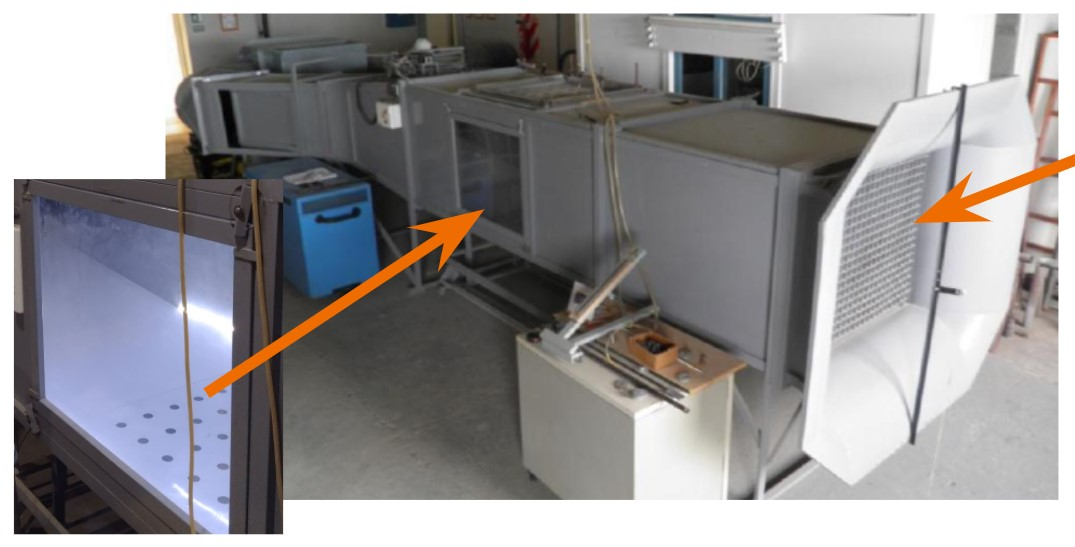
\includegraphics[scale=0.45]{remolinos.jpg}
	\captionof{figure}{Perforaciones dentro de la cámara de ensayos
		y "Panal de abeja"}
	\label{fig:remolinos}
\end{figure}


La figura \ref{fig:fluct} muestra, en este caso, las fluctuaciones alrededor de una velocidad media dentro de un tiempo específico. 
Para determinar la velocidad media se analiza un intervalo de tiempo suficientemente grande, de modo que el valor promediado en el tiempo se estabilice en una constante.
\begin{figure}[h!]
	\centering
	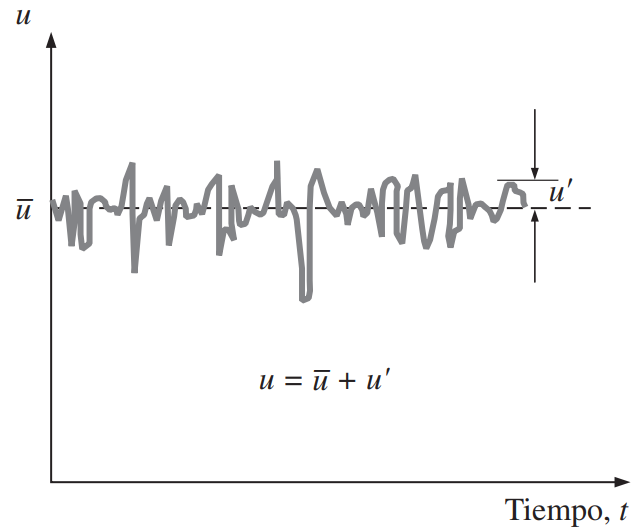
\includegraphics[scale=0.4]{fluct.png}
	\captionof{figure}{Fluctuaciones}
	\label{fig:fluct}
\end{figure}


\newpage
\section{Desarrollo}  \label{sec:desarr}

\subsection{Microcontrolador, sensores y comunicación}


\begin{tcolorbox}[colback=blue!5!white,colframe=blue!75!black,title=Microcontrolador] Es un circuito integrado programable, capaz de ejecutar las órdenes grabadas en su memoria. Está compuesto por unidad central de procesamiento (CPU), memorias (ROM y RAM), líneas de entrada/salida, módulos de comunicación, DAC, ADC, entre otros.
\end{tcolorbox}

\begin{tcolorbox}[colback=blue!5!white,colframe=blue!75!black,title=I$^2$C]
	Es un puerto y protocolo de comunicación serial, define la trama de datos y las conexiones físicas para transferir bits entre 2 dispositivos digitales. El puerto incluye dos cables de comunicación, SDA (Datos seriales) y SCL (reloj serial). Además el protocolo permite conectar hasta 127 dispositivos esclavos con esas dos líneas, con hasta velocidades de hasta 5 Mbps, 10 veces mayor que un puerto serial estándar. \end{tcolorbox}



	

Para la elección del microcontrolador se analizó varios dispositivos, como por ejemplo \textit{Arduino UNO}, \textit{Arduino MEGA}, \textit{Arduino NANO}, \textit{EDUCIAA}, entre otros. Se llegó a la conclusión que \textbf{Arduino NANO} era un microcontrolador de bajo costo, tamaño reducido, baja complejidad en la programación, con bibliotecas de diversos sensores y que cumplía con las prestaciones necesarias (señal de PWM, comunicación I$^2$C, entradas analógicas y digitales).

Como se nombró en la sección \ref{sec:ecvel}, es necesario tener mediciones de temperatura, humedad, presión atmosférica y diferencia de presión. Por lo tanto se realizó ensayos con diversos sensores en una protoboard comunicados con el microcontrolador por medio del protocolo de comunicación I$^2$C. Con las mediciones se eligió aquellos que generaron la menor variación de THP respecto a los instrumentos del laboratorio. 

Sensores utilizados
\begin{itemize}
	\item  \textbf{BME280:} Sensor de presión atmosférica, temperatura y humedad relativa.
\subitem \textit{Resolución de temperatura: 0.01 $^{\circ}C$}
\subitem \textit{Resolución de humedad: 0,008\% HR}
\subitem \textit{Resolución de presión atmosférica: $\pm$1hPa}
	
	\item \textbf{SHT21:} Sensor de temperatura y humedad relativa.
\subitem \textit{Resolución de temperatura: 0.01 $^{\circ}C$}
\subitem \textit{Resolución de humedad: 0,04\% HR}	
	
	\item \textbf{MPXV7002:} Sensor de presión diferencial.
\subitem \textit{Sensibilidad: 1 $V/kPa$}
\subitem \textit{Rango de presión: -2 $kPa$ a 2 $kPa$}	
	
	\item \textbf{ADS1115:} Convertidor analógico digital utilizado en conjunto con MPXV7002.
\subitem \textit{Resolución: 15 bits}
\end{itemize}


\begin{figure}[htbp]
	\centering
	\subfigure[BME280]{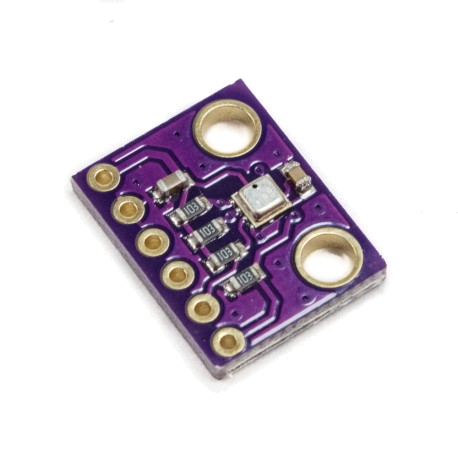
\includegraphics[width=25mm]{bme280.png}}
	\subfigure[SHT21]{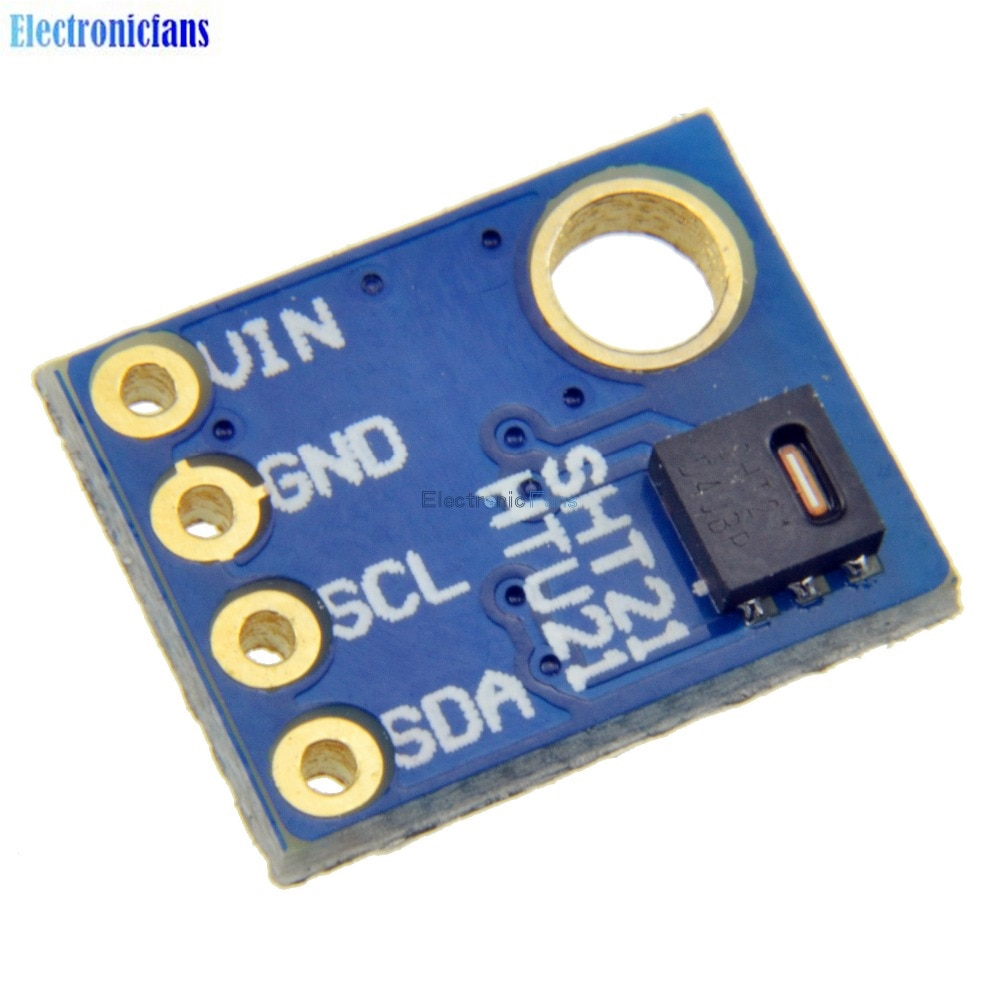
\includegraphics[width=30mm]{sht21.png}}
	\subfigure[MPXV7002:]{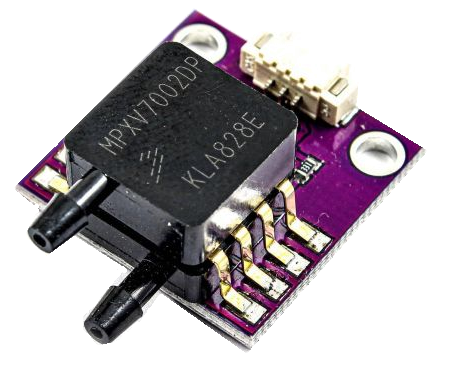
\includegraphics[width=30mm]{mpx7002.png}}
	\subfigure[ADS1115]{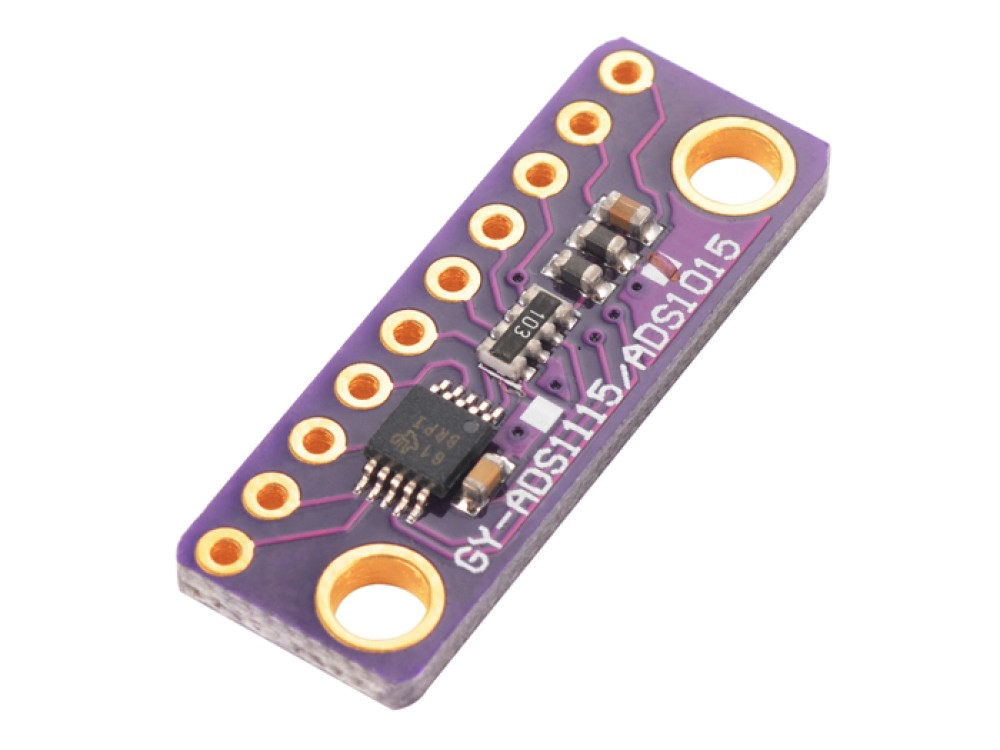
\includegraphics[width=35mm]{ads1115.png}}
	\caption{Sensores utilizados} \label{fig:senstodos}
\end{figure}




Se realizó ensayos para probar y corroborar el funcionamiento del \textbf{MPXV7002}, un sensor de diferencia de presión de alto costo en el país. Este sensor es capaz de medir de -2kPa a 2kPa en un rango de 4V (0.5 a 4.5V), al tener un único sentido de flujo, solo se necesitó medir valores positivos de presión.

Al tener una salida analógica se utilizó el conversor analógico/ digital ADS 1115. 
No se utilizó el ADC interno del microcontrolador Arduino ya que la resolución es de 10 bits y del ADS1115 de 15 bits.
También posee un amplificador de ganancia programable (PGA) que establece la escala completa, es decir, indica el valor de referencia. En Arduino este valor viene determinado por el voltaje de referencia que en el caso de Arduino NANO es 5V. En el ADS1115 lo establece el PGA. Por defecto este valor de referencia es ±6,144 V, quiere decir que el valor de 32.677 (valor máximo con 15-bit) corresponde a 6,144 V. 

Resolución en Arduino NANO:
\begin{center}
	\begin{math}Factor\;de\;escala=\frac{5\;V}{1023}=\;0,0048875\;V\;=\;4,88\;mV
	\end{math}
\end{center}

Resolución en ADS115:
\begin{center}
	\begin{math}Factor\;de\;escala=\;\frac{6.144\;V}{32677}=\;0,0001875\;V\;=\;0,1875\;mV
	\end{math}
\end{center}

En la tabla \ref{tab:Reso} se observa los valores posibles de factor de escala para distintos PGA. Este valor se eligió para aprovechar la mayor resolución posible al tener en cuenta el sensor utilizado.
\begin{table}[h]
	\centering
	\begin{tabular}{|c|c|c|}
		\hline
		\textbf{PGA} & \textbf{Referencia (V)} & \textbf{Factor de Escala (mV)} \\ \hline
		2/3          & 6,144                   & 0,1875                         \\ \hline
		1            & 4,096                   & 0,125                          \\ \hline
		4            & 1,024                   & 0,0312                         \\ \hline
		8            & 0,512                   & 0,0156                         \\ \hline
		16           & 0,256                   & 0,0078                         \\ \hline
	\end{tabular}
\caption{Factor de escala}
\label{tab:Reso}
\end{table}

En el caso de este proyecto, se utilizó un valor de PGA de 1, tomando como voltaje de referencia 4,096V.
\begin{center}
	\begin{math}
		Factor\;de\;escala=\;\frac{4,096\;V}{32677}=\;0,000125\;V\;=\;0,125\;mV
	\end{math}
\end{center}


\subsection{Adquisición de datos por puerto serie}
\begin{tcolorbox}[colback=blue!5!white,colframe=blue!75!black,title=Processing]
	\cite{processing}Es un lenguaje de programación basado en Java, aunque hace uso de una sintaxis simplificada y de un modelo de programación de gráficos.
\end{tcolorbox}
Para realizar la adquisición de datos por puerto serie, se utilizó en un primer momento Matlab, dónde, al realizar la comunicación con el microcontrolador, se guardaban los valores, pero estos no podían ser observados en tiempo real, sino que luego de las pruebas, se utilizaba otro script para obtener conclusiones. Luego de cierta cantidad de pruebas realizadas, se tornó indispensable observar los valores adquiridos, como la velocidad estimada en tiempo real.

Como solución para el inconveniente, se realizó una primera versión (Figura \ref{fig:Proce}) de un programa gráfico generado con Processing. Este código fue capaz de adquirir datos desde el microcontrolador en tiempo real y mostrarlos tanto gráficamente como numéricamente. 

Para realizar la estimación de la planta (Sección \ref{sec:estima}), era necesario poder implementar escalones de señal al variador de velocidad a través del microcontrolador. Esto fue posible ingresando valores numéricos por teclado que eran enviados al microcontrolador para generar la respectiva señal que luego sería ingresada al variador de velocidad por el modo de corriente (Sección \ref{sec:lazoI}).

Al presionar una tecla específica configurada por los comandos, el programa guardaba los datos adquiridos durante la prueba en un archivo .csv que luego fueron observadas con Matlab.

\begin{center}
	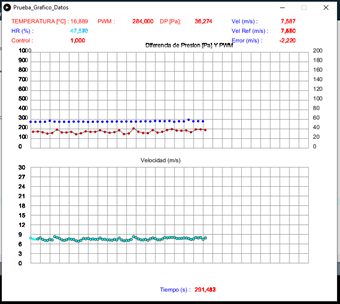
\includegraphics[scale=0.7]{serial_proc.png}
	\captionof{figure}{Pantalla Processing}
	\label{fig:Proce}    
\end{center}




\subsection{Filtros}
\begin{tcolorbox}[colback=blue!5!white,colframe=blue!75!black,title=Filtro digital]
	Un filtro digital, es un filtro que opera sobre señales digitales. Es una operación	matemática que toma una secuencia de números (la señal de entrada) y la
	modifica produciendo otra secuencia de números (la señal de salida) con el objetivo de resaltar o atenuar ciertas características.
\end{tcolorbox}

Una vez que se procedió a tomar diversos valores de velocidad estimada, se notó necesario la implementación
de un filtro. Para esto se utilizó varias bibliotecas preestablecidas de \textbf{Arduino} con las cuales se realizó la implementación de diversos filtros en el microcontrolador, con diferentes parámetros para posterior comparación (Figura \ref{fig:filtros}).


\begin{figure}[H]
	\centering
	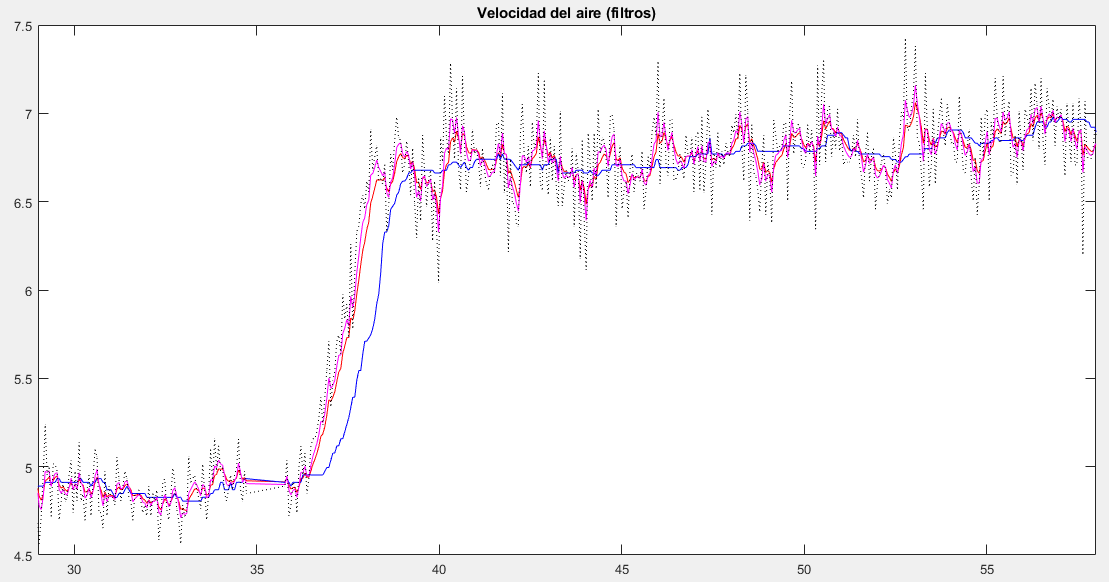
\includegraphics[scale=0.5]{filtros.png}
	\captionof{figure}{Datos y diversos filtros}
	\label{fig:filtros}
\end{figure}


\subsubsection{Filtro de mediana}
\begin{tcolorbox}[colback=blue!5!white,colframe=blue!75!black,title=Mediana]
	Es una técnica de filtrado digital no lineal que suele utilizarse para eliminar el ruido de una imagen o señal. La mediana es el número que está justo en el medio de un conjunto de datos ordenados de menor a mayor o de mayor a menor.
	La idea principal del filtro de mediana es recorrer la señal entrada, sustituyendo cada dato por la mediana de una ventana de “N” datos.
\end{tcolorbox}

Al observar y realizar la comparación de los filtros, se decidió utilizar el filtro de mediana (Figura \ref{fig:filtrosm}), con una ventana igual a 
40 muestras, que producía menor ruido en la estimación del aire. Como consecuencia del uso de este filtro, la señal se vió desfasada <10ms.

\begin{figure}[H]
	\centering
	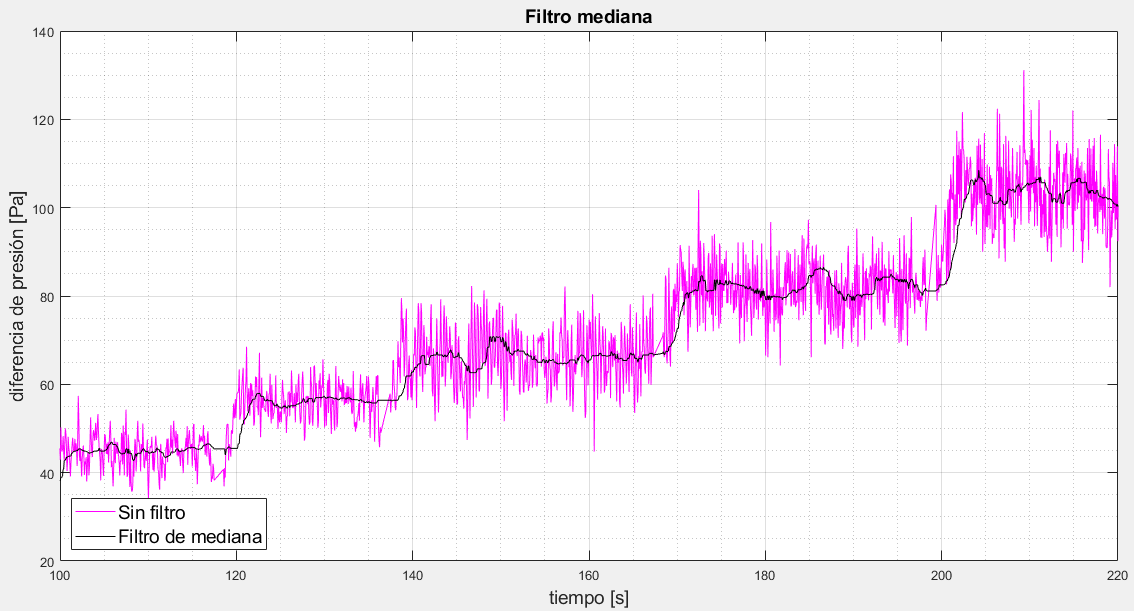
\includegraphics[scale=0.5]{filtro mediana.png}
	\captionof{figure}{Datos y filtro mediana}
	\label{fig:filtrosm}
\end{figure}



\subsection{Error observado}
Al utilizar el potenciómetro frontal del variador de velocidad u otro modo distinto al panel digital frontal, se originó un error en la aceleración o desaceleración.  Al hacer las averiguaciones pertinentes, esto se debió a una configuración interna del
variador y a las características propias del motor. \fcolorbox{red}{yellow}{ 3.2.2lubricación por cojinetes (y eliminarlo de ahí)}

Si el variador se utiliza con el panel digital frontal, la curva de aceleración y desaceleración
sigue una “s”, Figura \ref{fig:curvaS} no realizando un cambio brusco en la velocidad del motor, en cambio, para
el uso del potenciómetro u otro modo de funcionamiento la curva es lineal \ref{fig:curvarec}. Para revertir
esto, se modificó los parámetros del tiempo de aceleración y desaceleración del variador a 20 segundos.  


\begin{figure}[H]
	\centering
	\subfigure[Curva tipo s]{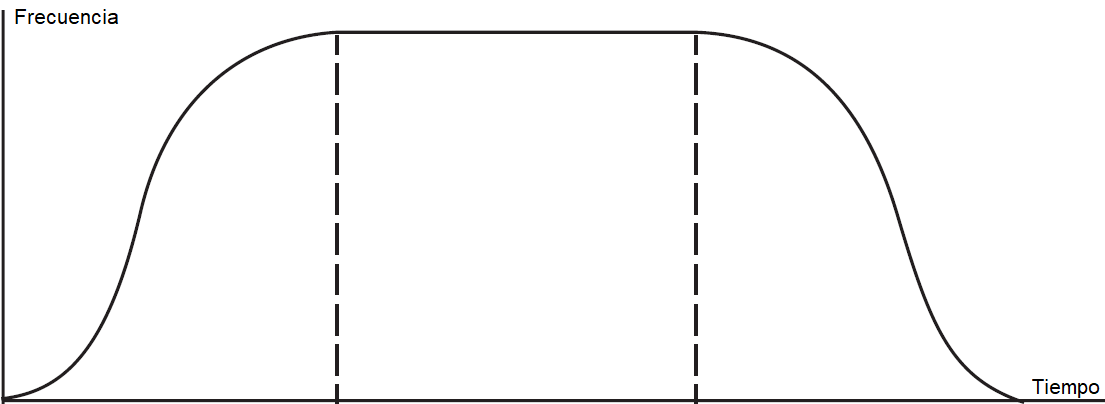
\includegraphics[width=60mm]{conS.png} \label{fig:curvaS}} 
	\subfigure[Curva tipo lineal]{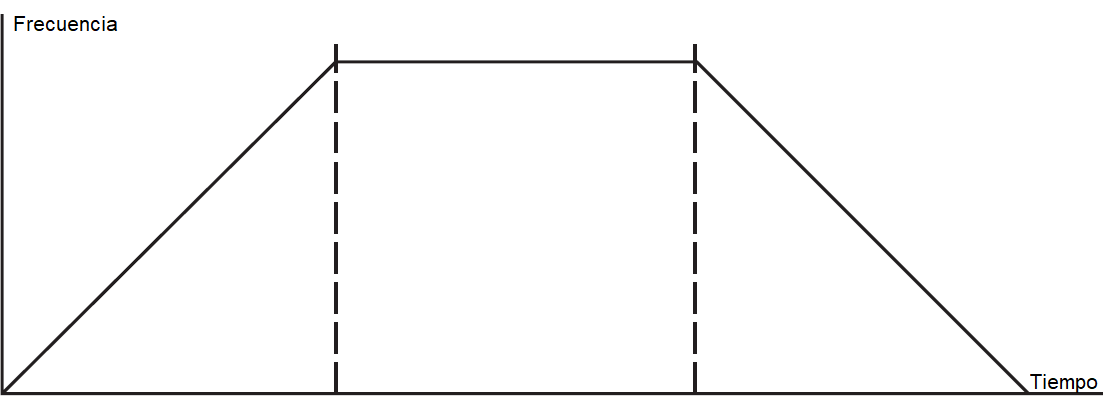
\includegraphics[width=60mm]{sinS.png} \label{fig:curvarec} }
	\caption{Curva aceleración y desaceleración} \label{fig:curva}
\end{figure}




\newpage